%\section{Racket Refactoring Tool}
%This section explains the decisions made in order to make this refactoring tool.

\section{Architecture}
%Refactoring Tool work flow: (add a brief explanation of what does)

%FIXME The Chosen IDE here??

In order to create correct refactoring operations, the refactoring tool uses two sources of
information, the def-use-relations and the AST of the program.
The def-use-relations are visually represented in a form of Arrows in DrRacket.
That information is especially relevant for refactoring operations such as Extrac-Function,
Add-Prefix, Organize-Imports, etc.

The AST is represented by the syntax expressions (s-exp) which composes the racket program.
In Racket everything is a syntax-expression and therefore accessing the list (tree)
of the syntax-expressions has all the information that a normal AST provides. %FIXME incorrect



\begin{figure}
\centering
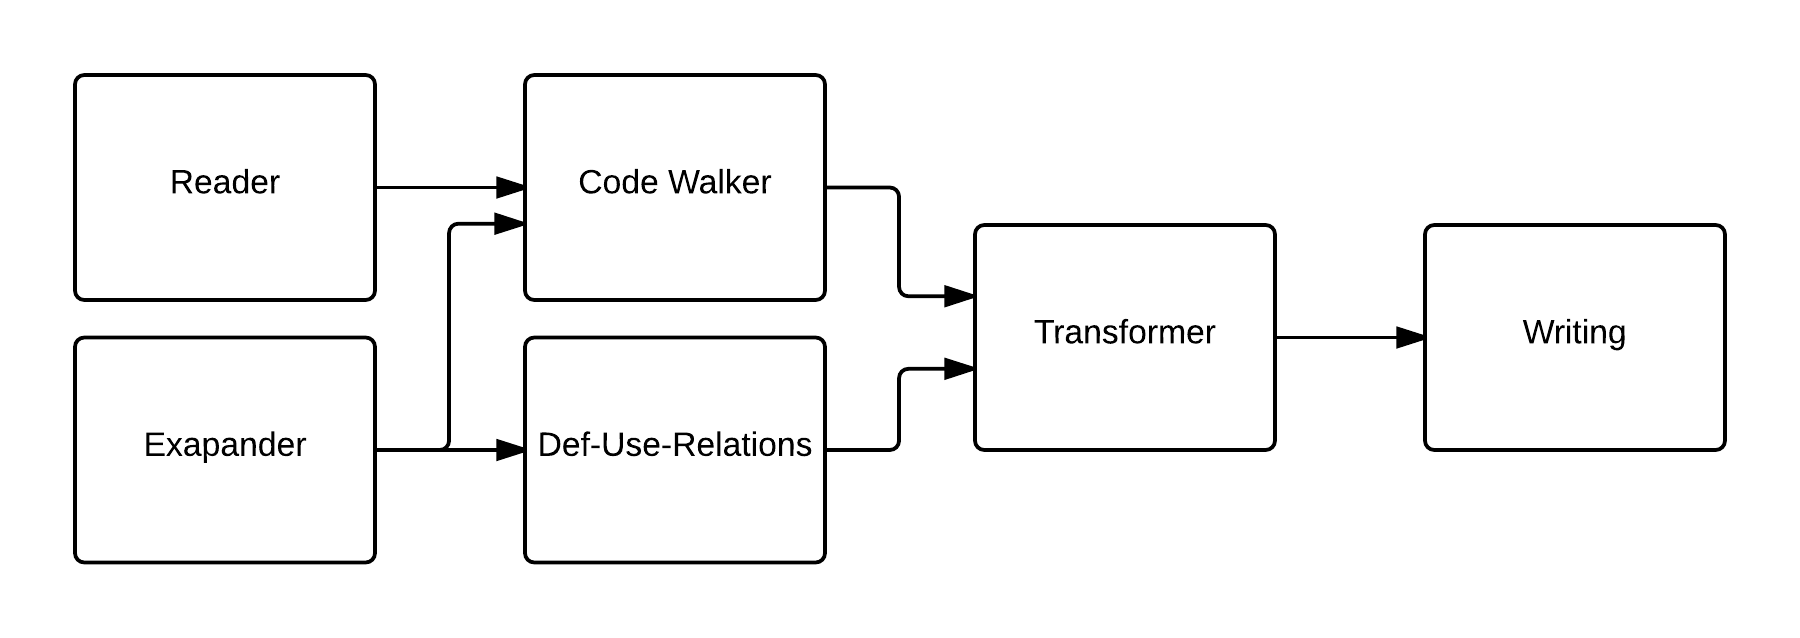
\includegraphics[width=\linewidth]{refactoringTool-arch.png}
\label{architecture}
\caption{Information flow between modules.}
\end{figure}
Figure~\ref{architecture} summarizes the work flow of the refactoring tool where
the Reader produces the non expanded program while the Expander produces the
expanded program. Afterwards the Code walker parses the AST produced by the Reader or the Expander depending the
cases. In order to produce the Def-Use-Relations it is necessary to use the code produced by the
Expander because it has the correct dependency information.
The Transformer uses both information from the Code Walker and the Def Use Relations
to transform the code. Then it goes to the Writing module that produces the output
in the Definitions area.

%The AST is acquired after using the check-syntax button. It was intended to be
%acquired automatically, because DrRacket has an online check syntax, but it was
%not possible. After that it cleans the AST removing information that is not
%necessary, at least for now, for the refactoring operations. When the AST is cleaned it
%passes the exact part of the AST that was selected. And tries to match rules,
%using syntax-parse against that syntax.

\subsection{Syntax Expressions}
%intro and explain the importance of the S-Exp
The s-exp list represent the AST, which provides information about
the structure of the program.
The s-exp list it is already being produced and used by the Racket language and
in DrRacket.
They represent the program and are computed in order to provide error information
to the user.
DrRacket already provides functions which computes the program's s-exp list and uses some of those
functions in the online check syntax and in the check syntax button callback.

%TODO add the functions?


\subsubsection{Syntax Expression tree forms}
DrRacket provides functions to compute the s-exp list in two different formats.
One format is the expanded program, this format is used by the Check Syntax and
the online check syntax, and computes the program with all the macros expanded. %maybe check that
The other format is the non-expanded program and computes the program with the macros
unexpanded.

The expanded program has the macros expanded and the identifier information correctly
computed.
However it is harder to extract the relevant information when compared with the
non expanded program.
%Racket has two forms of syntax tree. An expanded form, with the macros expanded
%and a non expanded form that is after a read-syntax without the macros expanded.

For example, the following program is represented in the expanded program,
and in the non expanded program. %FIXME TODO FIXME change example to a and, or, when or unless

\begin{lstlisting}[basicstyle=\ttfamily, caption="example"]
(and #f #t)
\end{lstlisting}

\begin{lstlisting}[basicstyle=\ttfamily, caption="Expanded program"]
#<syntax:2:0
 (#%app call-with-values
  (lambda () (if (quote #f)
   (quote #t) (quote #f)))
   print-values)>
\end{lstlisting}

\begin{lstlisting}[basicstyle=\ttfamily, caption="Non expanded program"]
#<syntax:2:0 (and #f #t)>
\end{lstlisting}
%Expanded Program Vs Not expanded Program
%Talk about difficulty, durability, Python (other languages)

%[Only in the expanded form] (and) is treated like an if which is bad and give problems
%The rest tends to work.
%testing:
%(if (= (+ 1 2) 1) \#f \#t) to (not (= (+ 1 2) 1))

The expanded program transforms the "and", "or", "when" and "unless" forms into
ifs and that makes refactoring operations harder to implement.

Racket adds internal representation information to the expanded-program which for
most refactoring operations are not needed.

However, the expanded program has important information regarding the binding
information that is not available in the non-expanded form and is rather useful
to detect if two identifiers refer to the same binding.
%TODO check; It also contains information where a program returns or not. TODO CHECK!
In addition, the expanded program has a format that is likely to change
in the future.
Racket is an evolving language and the expanded form is a low level and internal
form of representation of the program. %thus all improvements or changes in meaning will directly impact this representation

Therefore it is desirable to use the non expanded form for the refactoring %all things considered
operations whenever possible and use the expanded form only for the necessary
operations.


%Sub Cap Code with Macros The Problem
Macros usage could make the refactoring operations incorrect by modifying the   %FIXME rewrite
program behavior.
However, since the refactoring tool is targeted at unexperienced programmers macros
will not be used often and therefore it is not considered part of the scope of
this refactoring tool capabilities.
Nevertheless, if we intended to create a tool that gives support to refactoring macros
using the non expanded program would let to errors making the expanded program the
representation of the program used.
However, there are no guarantees that would be enough to ensure the correctness of
such refactoring operations due to the reflection capabilities of Racket.

%Dependency of Racket evolution
%Using the expanded program might simplify the refactoring for other languages,
%for example it has a literal that says when the program returns in python, and
%racket does not have it. In the expanded form there is syntax that explicitly says
%where the program returns.

%In the future it is possible to create a tool that uses both program expansions,
%making it possible to have macros and the relation with other languages for the
%more difficult problems and using the non expanded program for the simple cases.


\subsection{Def-Use-Relations}
Def-Use-Relations holds an important information in order to produce correct refactoring operations. %the def-use-relations? holds?
They can be used to check whether or not there will be a duplicated name
or even to compute the arguments of a function to be extracted.
%The information is computed in the online-comp.rkt that is where expands
%and computes the information needed to know the def-use-relations and whether
%the program is syntactically correct.
%There is an online expansion monitor that calls the online-comp, the online-comp
%then expands the program (to the expanded program) and does a trace to get the
%information needed for the arrows (def-use-relations).
%Afterwards it sends back that information to the caller of the online-comp to do
%the replay of the trace did by the compile comp and to process the information
%about the arrows.
%\subsubsection{Def-Use-Relations utility}
DrRacket already uses the def-use-relations in the system and they are visually  %TODO they are or it is?
represented by arrows in the GUI.
The def-use-relations is computed by the online-compiler that runs in the background.
However it is only processed when a program is syntactically correct. (e.g. if
a program has syntax errors there are no arrows produced in DrRacket)

\subsection{Code-walker}
The code-walker is used to parse the syntax tree represented by a syntax elements
that is a list of s-exp in racket. %TODO check this.
A syntax element can contain either a symbol, a syntax-pair, a datum (number, boolean or string),
or an empty list. %might be other stuff but never got it, not relevant?
While a syntax-pair is a pair containing a syntax object as it first element and
either a syntax pair, a syntax element or an empty list as the second argument.
Each syntax-object has information about the line where they are defined and this
information is to search for the correct elements.

%A syntax object combines a simpler Racket value, such as a symbol or pair, with a scope set at each phase level,
%source-location information, syntax properties, and tamper status. In particular, an identifier is represented as
%a syntax object that combines a symbol with scope sets and other information. The lexical information of a syntax
%object is its scope set combined with the portion of the global table of bindings that is relevant to the syntax object’s set of scopes.

Most of the time using the code-walker we are searching for a specific syntax element
and location information contained in the syntax-object  is used to skip the syntax
 blocks that are before the syntax element wanted in the first place.

The Code-walker is a core part of the refactoring tool ensuring that the selected
syntax is correctly fed to the refactoring operations. %actually?

%the way that the code-walker guarantees that goes to every important part of the
%tree is by having a "pointer" to the current selected syntax element, and have
%a stack that contains the remaining code to analyze.
%Because of this structure it is necessary to have a stack in order to search
%the tree correctly and in the best way possible.
%Because Most of the time we are searching for a specific syntax element (e.g function,
%define, etc, because everything is a syntax element in Racket) and using this we
%can skip uninteresting syntax in order to get to the syntax that we want to use.


%%%%%% Writing Part of the Refactoring/refactoring rule
\subsection{Pretty-printer} %output?
%FIXME comments, how to solve this?
Producing correct output is an important part of the refactoring tool.
It is necessary to be careful to produce indented code and we decided to use a pretty-printer
that is already incorporated in the language.
However this pretty-printer does not follow the convention in the cond clauses
should be surrounded by [ ] parenthesis. This is not considered a problem because
Racket supports both representations.
One possible solution is to use a different pretty-printer in
order to keep the language convention.

%Some syntax elements (s-expressions) lose some information about parenthesis.
%For example it is a convention that cond clauses should be surrounded by [] parenthesis
%but the syntax element does not store that kind of information.
%There are several pretty-printers developed for Racket and even the Racket language
%has one incorporated.
%The one already incorporated does not use the [ ] parenthesis, however racket
%supports both representations.
\subsection{Comments preservation}
Preserving the comment after a refactoring transformation is an important task
of the refactoring tool. If the comment in determined place of the program
changes hits location affecting another structure it could confuse the programmer.
However comment preservation is not implemented yet, making it a limitation of
this prototype.

One possible solution is to modify the syntax reader and add a comment node to the
AST.
While the new node will not be used during refactoring transformations it is used
during the output part of the refactoring operation preserving the comment with
the correct syntax expression.


\subsection{Syntax-Parse}

The Syntax-Parse function provided by Racket is rather useful for the refactoring
operations regarding mainly syntax information.
It provides a wide range of options to help matching the correct syntax with  %fine tunning
backtracking.
The backtracking it is possible to have several rules to be matched
in the same syntax parser, which helps to create more sophisticated rules.

\section{Refactoring operations}
%TODO do introduction
In this section we explain some of the  more relevant refactoring operations and
some limitations of the refactoring tool.

\subsection{Semantic problems}
There are known semantic problems that might occur after doing a refactoring
operation.
One problem occurs when removing the and of the following example.

\begin{lstlisting}[basicstyle=\ttfamily, caption="And example"]
  (and (< 1 (foo 2)) (< (foo 2) 3))
\end{lstlisting}
The refactoring transforms the code into this:
\begin{lstlisting}[basicstyle=\ttfamily, caption="Example"]
  (< 1 (foo 2) 3)
\end{lstlisting}

\begin{lstlisting}[basicstyle=\ttfamily, caption="Foo"]
(define (foo arg)
  (displayln "foo"))
\end{lstlisting}

Instead of applying the side effect that is displaying the the string "foo"
 it will only display the it once. Therefore changing the meaning of the program.

We still kept this refactoring operation because in the vast majority
of the cases this refactoring operation does not change the semantic of the program.
Furthermore, the possible solution would limit excessively this refactoring operation.  %enormously
Considering Racket's reflection capabilities we would only apply this refactoring operation
safely when the arguments of the function, in this case " < " were datums (number, boolean or string). %FIXME

\subsection{Extract Function}
Extract function is an important refactoring operation that every refactoring tool
should have.
However there are some concerns to have into account.
In order to extract a function it is necessary to compute the arguments needed
to the correct use of the function.
While giving the name to a function seams quite straightforward it is necessary to
check for name duplication in order to produce a correct refactoring. (e.g. having
two identifiers with the same name, in the same scope produces an incorrect program
and therefore modifying the meaning of the program).
%TODO we assume that the program is correct before applying the refactoring operation
Then computing the body and replacing it by the call should be straightforward.
Another problem is where should the function extracted to. A function can not
be defined in an expression, (e.g inside a let) but it could be defined in the top-level
or in any other level that is accessible from the top level.

e.g: When extracting the \'(+ 1 2) to a function where should it be defined?
Top-level? level-0 level-1 or in the current level, level-2?
\begin{lstlisting}[basicstyle=\ttfamily, caption="Extract function levels"]
;;top-level
(define (level-0)
  (define (level-1)
    (define (level-2)
      (+ 1 2))
    (level-2))
  (level-1))
\end{lstlisting}

The fact is that is extremely difficult to know the answer to this question because
it depends on what the user is doing and the user interpretation.
Accordingly we think that the best solution is to let the user decide where
he want the function defined.


\subsubsection{Computing the arguments}
%In previous versions of the online-comp information about the type of arrows
%was available in the structure. However in the recent versions that type of
%information was removed.

%With the previous version of the online-comp the framework was computing the argument for the
%newly extracted function using the type information: "one of 'lexical, 'top-level, 'import".
In order to compute the arguments we have to know in which scope the variables are being defined, in other words,
if the variables are defined inside or outside the extracted function. %FIXME it is weird
The variables defined outside the function to be extract are the candidates to be the argument %FIXME IMPROVE
of that function, however imported variables, whether from the language or from other libraries
does not have to be passed as arguments.
%There are no information in the def-use-relations that indicates whether an variable is imported or not.
We considered two possible solutions:

  -Def-use-relations + Text information

  -Def-use-relations + AST

The first approach is simpler to implement and more direct than the second one.
However it is less tolerant to future changes and to errors.
The second one combines the Arrow information with the syntax information to
check whether it is imported from the language or from other library.

We choose the second approach in order to provide a more stable solution to compute
 correctly the arguments of the new function.

\subsection{Let to Define} %implemented is it worth it?
%Refactoring Let to Defines Usefulness Vs implementation difficulty
%TODO implement
Changing a let form to a define could be rather useful when the user
notices that instead of a let form it should be a function. %FIXME missing commas?

%let* vs let
There are several types of let forms, but the most common are the let and the let*.
There is a subtle difference between this two keywords that influences directly the simplicity of the solution.
The let defines variables independently, while let* can use the value of the variable defined before.

\begin{lstlisting}[basicstyle=\ttfamily, caption="let form"]
(define a 10)
(let ([a 1]
      [b (+ a 1)])
      ...
      )
\end{lstlisting}
The let defines the variables independently thus the value of b is 11.

\begin{lstlisting}[basicstyle=\ttfamily, caption="let* form"]
(define a 10)
(let* ([a 1]
      [b (+ a 1)])
      ...
      )
\end{lstlisting}
However in the case of let* the value of b is 2.

%Therefore only the let would be considered because it is a more directly
%representation of a function.

%named let.
Named let is a let that has a name and can be called, like a function.
The named let is directly mapped as a function and therefore might be useful to transform to a function.
The same applies from a function to a named let.
However this has a problem, a let form can be used in expressions, but the define can not.
In the vast majority of cases this refactoring is correct, but when a let is used in an expression
it is not correct and it changes the meaning of the program, transforming a correct
program in a incorrect one.
e.g.
\begin{lstlisting}[basicstyle=\ttfamily, caption="Let in an expression"]
(and (let* test ((a 1)) (< a 2)) (< b c))
\end{lstlisting}
Modifying this named let into a define would raise a syntax error because a
define could not be used in an expression context.

This could be solved by using the local keyword that is an expression like
the let form.
However the local is not used very often and can confuse the users. This reason
made us keep the refactoring operation without the local keyword that works for
most of the cases.


%\subsection{Define to Let} %not yet implemented
%Refactoring Define to Let Usefulness Vs Implementation difficulty
%TODO implement.
%Useful for when changing several defines and merging them into a let.
%the let would "swallow" all the range of the defines scope
%Interesting?

%It would be let* and named let* If define is a function it does not work.
%Is that worth it?

\subsection{Wide-Scope Replacement} %is this a feature or a refactoring?
The Wide-Scope replacement brings the possibility to replace all the duplicated
code with a function call. This is usually performed after an extract function refactoring.
%The Wide-Scope Replacement brings an huge improvement on the utility of the refactoring regarding the use
%of the extract function refactoring operation.

The Wide-Scope replacement refactoring operation searches for the code that is duplicated of the extracted function and then it replaces for the call of the
extracted function and it is divided in two steps: %FIXME Improve

- Detect duplicated code

- Replace the duplicated code

Replacing the duplicated code is the easy part, however the tool might has to compute %have?
the arguments for the duplicated code itself. The argument computation occurs when
the code is the same, but it has different variable names. This is not yet in this
version of the refactoring tool. %TODO rewrite, it is buggy

\subsubsection{Detecting duplicated code}
Correctly detect code duplication is a key part for the correctness of this refactoring.
Even the simplest form of duplicated code detection, when it only detects code duplication
when the code is exactly equal, may have some problems regarding the bindings.
For example, if the duplicated code is inside a let that changes some binding that must
be taken into consideration.
Racket already provides functions that compute if the bindings are the same.
However that does not work if we consider the program in the not expanded
form because there is not enough information for those bindings to work. %FIXME improve :(

%[TODO Recently racket changed binding expansion and it brought interesting improvements to racket and that might be useful for this, read paper before]

Therefore, in order to compute the correct bindings, it is necessary to use the expanded form
of the program.

The naive solution is to use the expanded program to detect the duplicated
 code and then use this information to do the replacing of the duplicated code.
However when expanding the program Racket adds necessary internal information to
run the program itself that are not visible for the user.
While this does not change the detecting of the duplicated code, this adds unnecessary information
that would have to be removed. %FIXME
In order to solve this problem in a simple way we can use the expanded code to detect
the correctly duplicated code and use the non expand program
to compute which code will be replaced.

However this detection is a quadratic algorithm which might
have some performance problems for bigger programs. %TODO TODO TODO

Detecting duplicated code can be added to the automatic detection of possible refactoring operations to be applied. %FIXME is this already done?
Notifying the users of a possible extract function operation if there is duplicated code.
This is a rather useful notification because for programs that are bigger than the
visible part of the screen.
Which might be difficulty for the user to remember if a piece of code was duplicated or not.


%This runs after detecting the duplicated code, so the bindings are corrected identified.

\subsection{Ambiguities}
There are some cases where two types of syntax refactoring apply.
E.g.:
\begin{lstlisting}[basicstyle=\ttfamily, caption="Code sample"]
(if ?x
    (begin ?y ...)
    #f)
\end{lstlisting}
The two different refactoring transformations are possible:
\begin{lstlisting}[basicstyle=\ttfamily, caption="Refactoring option 1"]
(when ?x
      ?y ...)
\end{lstlisting}

\begin{lstlisting}[basicstyle=\ttfamily, caption="Refactoring option 2"]
(and ?x (begin ?y ...))
\end{lstlisting}

The programmer may want in some situations choose one approach and in others
choose the other one. For example if a programmer is creating a predicate may
choose the "and" version, whereas if the programmer is using another control structure
may prefer the "when" version.

This example shows how hard it is to have an semi-automated refactoring tool
that gives suggestions.
It could displays both possibilities, but that will create an precedent meaning
that if a refactoring has several possibilities the tool has to display every one.
Or it could only display that there is a refactoring opportunity.
This requires further reflection to choose the best approach to the problem.


%\subsection{Implemented Refactoring Operations:}
%Is this worth it?
